\section{Codes' set up}

At this point, it is clear that I took many consecutive steps to model mass transfer in triple systems with a Roche-lobe filling outer star. A schematic representation of the entire process is provided in \cref{fig:schematic_method}
\begin{figure}[H]
    \centering
    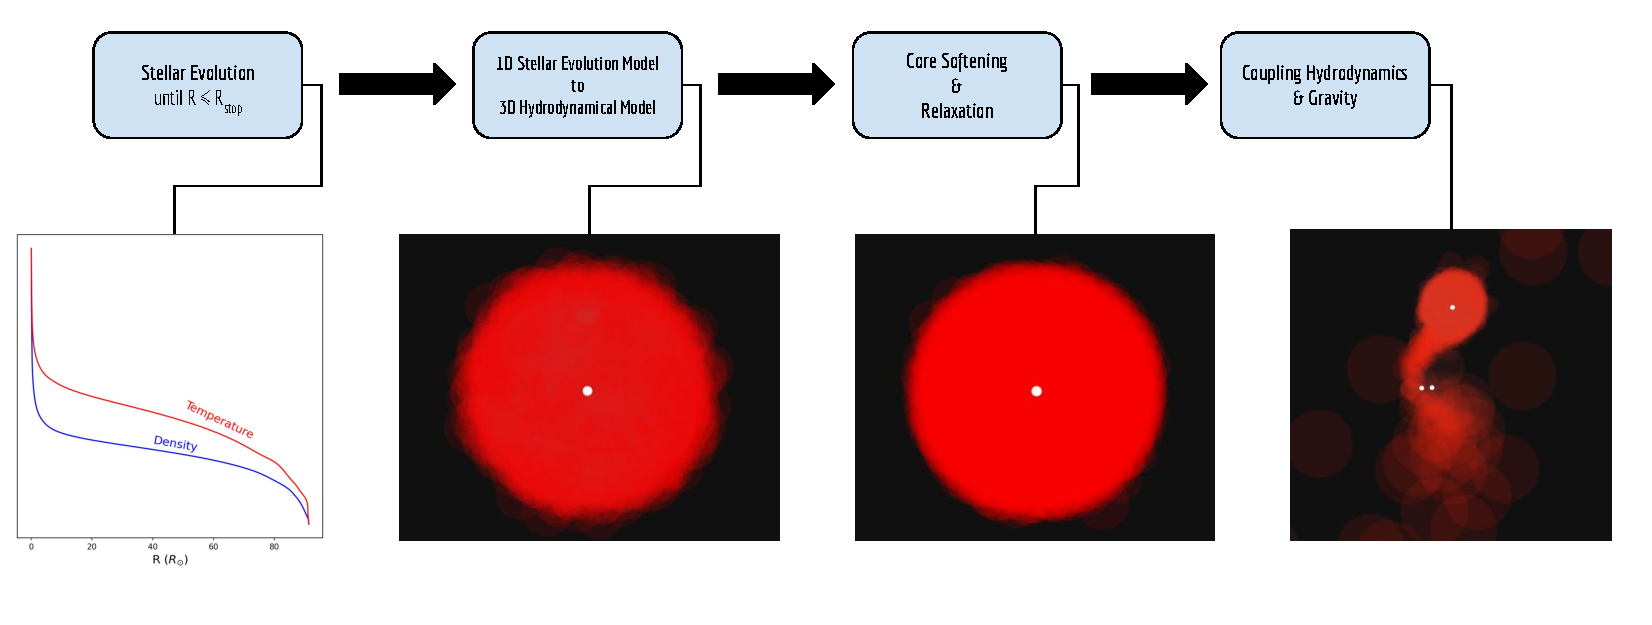
\includegraphics[width=\textwidth]{Thesis/figures/method_schematic.pdf}
    \caption{Schematic representation of the steps taken to simulate mass transfer in the triple system with a Roche-lobe filling outer star. The white points are the purely gravitational particles representing the core and the inner binary components. The red points are the \ac{sph} particles representing the gas having an adaptive smoothing length.}
    \label{fig:schematic_method}
\end{figure}
In each step, I explored the importance of different parameters and made assumptions based on relative physics to better simulate the system's behavior. The outcome of a simulation is, of course, dependent on the simulation's setup; Furthermore, knowing the setup parameters is important for the reproducibility of the results. Hence, I summarize the codes' settings used for the final simulations for the reader.
\begin{table}[H]
    \centering
    \begin{tabular}{ |p{6.5cm}||p{6.5cm}|  }
     \hline
     \multicolumn{2}{|c|}{Code Settings} \\
     \hline
     MESA & GADGET-2 \\
     \hline
     Initial Masses = [3.2, 3.1. 5.5] M$_{\odot}$& $N_{particles}=50^4$ \\
     Solar metallicity& Self-gravity: True\\
     No winds& Adaptive smoothing length: True\\
     No overshooting& Softening = smoothing length\\
     No star rotation & Adiabatic \ac{eos}  \\
     Convection-occurrence (Schwarzwild) & Time step = $1/64 \times P_{in}$ \\
     Evolve until $\geq 1.1 \times R_{RLOF}$ & Artificial viscosity: $\alpha=0.5, \beta=1.0, \eta=0.1$ \\
     \hline
    \end{tabular}
        \centering
    \begin{tabular}{ |p{6.5cm}||p{6.5cm}|  }
     \hline
     \multicolumn{2}{|c|}{Code Settings} \\
     \hline
     Huayno & AMUSE \\
     \hline
     No softening length & Gravity-Hydrodynamics (2nd-order-coupling)\\
     Default time step ($<< 1/64 \times P_{in}$) &  Bridge time step = $1/64 \times P_{in}$\\
     \hline
    \end{tabular}
    \caption{ Various important settings and flags used for the different codes and AMUSE}
\label{tab:codes_settings}
\end{table}
